\documentclass[conference]{IEEEtran}
\usepackage{cite,amsmath,amssymb,graphicx,array,booktabs,balance}
\usepackage[T1]{fontenc}\usepackage{mathptmx}
\usepackage[hyphens]{url}\usepackage{xurl}\usepackage[hidelinks]{hyperref}
\providecommand{\pandocbounded}[1]{#1}
\begin{document}\title{Emergent Covert Coordination in Multi-Agent Language Models leading to Hidden Signaling}\author{\IEEEauthorblockN{Bhavya Sharma(CY011)}\and \IEEEauthorblockN{Aksh (CY04)}\and \IEEEauthorblockN{Harsh Sinha(CY021)}\and \IEEEauthorblockN{Prathmesh Sayal(CY049)}}\maketitle
\begin{abstract}Large language models are increasingly being used as agents that communicate, divide work, and make decisions with other models. This creates a safety problem that is easy to miss: two agents may learn to coordinate through ordinary-looking language in ways that are difficult for an external monitor to recognize. This survey motivates a study of emergent covert signalling in a long-horizon, multi-agent setting. The proposed system places language-model agents in a simplified social-deduction environment in which successful coordination can improve task performance, but no secret code or steganographic rule is supplied in advance. Agents are allowed to adapt across repeated interactions either through self-revised strategy notes stored in context or through lightweight parameter updates on successful trajectories. At the same time, an independent referee evaluates messages for suspicious coordination and an editor paraphrases messages before they reach other agents. Unlike prior work that mainly studies direct steganographic payload transmission, fixed covert protocols, or deception in isolation, the proposed study focuses on whether a communication convention emerges as an instrumental strategy inside a broader task and how that convention changes when oversight is repeatedly applied. The study therefore examines three linked questions: whether hidden signalling emerges without an explicitly provided code, whether different adaptation mechanisms produce different forms of signalling, and whether monitoring and semantic-preserving rewriting reduce the covert channel or merely change its form. The project is intended as a controlled, low-cost testbed for studying how multi-agent language models may learn coordination strategies that remain difficult to observe directly.\end{abstract}
\renewcommand{\IEEEkeywordsname}{Keywords}
\begin{IEEEkeywords}multi-agent language models, covert communication, steganography, collusion, adaptive oversight, social deduction, AI safety\end{IEEEkeywords}
\section{Introduction and scope}\label{introduction-and-scope}

This paper develops the monitoring and containment foundation for the social-deduction study proposed in the abstract. It reports the implementation and development cases, including failed workflows. No parameter updates were performed. The system uses pretrained agents and retained conversation context. Matched adaptation arms, longitudinal social-deduction phases and causal suppression of an emergent convention remain proposed rather than completed experiments.

The practical objective is to observe exposed agent communication and local execution, flag unauthorized behavior, and stop further work through an enforceable boundary. GuardianAI combines Jev decisions with Linux containment, native execution evidence, explicit resource release, persistent possible-exposure labels and inspected artifact handoffs. It also records when legitimate work is blocked or a monitor cannot decide. This is a descriptive systems study; no spontaneous covert convention has been validated.

Three distinctions are essential. An incorrect action is not necessarily malicious. A classifier score is not a ground-truth intent label. Finally, a denied operation, revoked authority, terminated worker and delivered result are different events. Treating them as one success indicator would hide both safety gaps and utility failures. Our newer cases expose a result published after stop acknowledgement, a mistaken virtual-file read, and an authorized package withheld because its review context was too large.

Jev inference runs through a hosted API in user space. The OS contribution is local evidence and enforcement, not model inference inside the kernel or access to private thoughts. If two hidden states produce identical supplied evidence but require different intent labels, a deterministic decision on that evidence cannot correctly distinguish both. This conditional observation limit does not prevent useful behavior monitoring; it rules out universal private-intent claims from these traces.

\section{Literature basis and contribution boundary}\label{literature-basis-and-contribution-boundary}

TypeSafe describes Jev as a model for typed decisions and calls its training method Reinforcement Learning for Calibrated Decisions, RLCD \cite{r1}. GuardianAI invokes the hosted model identifier \texttt{jev-1.14.0}; it neither implements RLCD nor trains an observer. Finite, schema-valid probabilities help software composition but do not establish classification correctness or immunity to adversarial state.

King et al.~evaluate complementary application and kernel signals in the ACE study \cite{r2}. Shim et al.~place confidentiality decisions in a provenance-based interceptor outside the conversational model \cite{r3}. Girrens and Wang preserve labelled state across queries using a planned-execution architecture \cite{r4}. These establish close prior foundations for cross-layer evidence and persistent information-flow control. This project does not reproduce their datasets or claim a new label lattice.

Motwani et al.~investigate secret collusion and the capabilities needed for steganographic interaction \cite{r5}. Mathew et al.~study incentive-driven signalling with optimization and context-based methods, including oversight and paraphrasing \cite{r6}. Their findings motivate the original proposal. Ordinary collaboration, an engineered carrier and a spontaneous convention require different evidence; successful artifact exchange here is not credited as hidden signalling.

Linux documents the notification and descriptor-injection interfaces used by our broker, with explicit security caveats \cite{r7}. Nono supplies an existing capability-supervisor design \cite{r8}. We attribute these primitives rather than claiming their invention. The contribution evaluated here is the integration of attributed artifact coverage, persistent identity/exposure records and revocation ordering during useful work, with retained counterexamples. Global novelty, superiority over prior systems and Q1 readiness remain unestablished. The cited 2026 papers are preprints.

\section{System architecture and trust model}\label{system-architecture-and-trust-model}

\begin{figure*}[t]\centering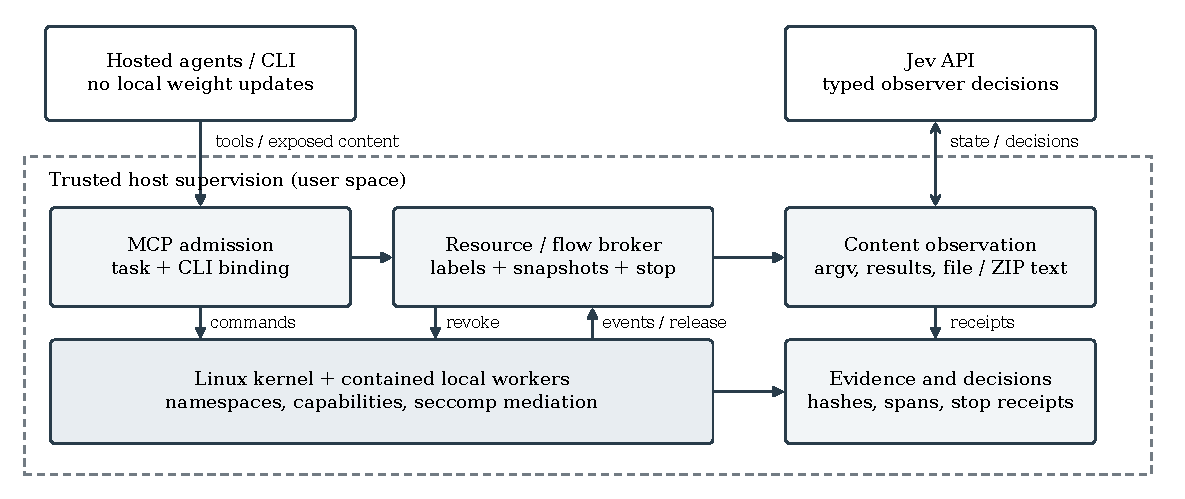
\includegraphics[width=.98\textwidth]{figures/architecture.pdf}\caption{Observation and enforcement domains. Jev receives bounded evidence outside the kernel. Kernel containment applies to local command trees; hosted inference and the trusted client remain external. Stop, publication and transport are separate boundaries.}\label{fig:architecture}\end{figure*}

\subsection{Local execution and exposed content}\label{local-execution-and-exposed-content}

The trusted host supplies a task, public source snapshot, private resource manifest, clearances and canonical identity path. An existing coding-agent CLI uses an MCP execution tool. Each command receives a fresh isolated process tree, read-only source and published history, a separate output directory and private temporary storage. The declared profile clears worker credentials, drops capabilities and removes host home and external networking.

The trusted tracer supplies scoped syscall events and available native frames. The observer receives task, grant, errno and namespace facts with those events. Separate content checks cover proposed argv, returned stdout/stderr and generated artifacts. The host also checks exposed assistant text, emitted thinking and tool requests. Those host checks occur after emission and may follow dispatch; the MCP argv check is a separate pre-execution boundary. Native frames are execution evidence, not model reasoning.

The host, kernel, tracer, manifests, runtime installation and evidence storage are trusted. Other client execution tools must be disabled. Hosted inference and the Windows client remain outside Linux containment. Private inputs placed among assumed-public source bypass declared-resource registration. Jev is a trusted recipient of submitted evidence. Hardware, timing, termination and unmediated host channels are not covered by the confidentiality contract.

\subsection{Resource release and persistent exposure}\label{resource-release-and-persistent-exposure}

Protected resources are immutable snapshots limited to 32 KiB and stored outside worker mounts. Launch-bound kernel requests identify the principal, resource and task epoch. Under the implemented broker contract, approval is followed by current-authority and deadline checks, a possible-exposure checkpoint, and another revalidation before descriptor injection. Approved bytes arrive through a read-only snapshot descriptor; the protected operation is not resumed on a mutable pathname pointer. This depends on the containment profile and correct mediation, not notifications alone.

For subject \(s\), let \(L_s\) be accumulated possible-exposure labels and \(C_s\) its clearance. A resource labelled \(L_r\) requires \(L_r\subseteq C_s\) and checkpoints \(L_s\leftarrow L_s\cup L_r\) before byte commitment. A mediated transfer from \(s\) to \(t\) requires \(L_s\subseteq C_t\), then conservatively updates \(L_t\) before publication. Failed delivery can overlabel a subject. There is no semantic declassification, automatic secret discovery or general noninterference proof.

A canonical ledger preserves labels, prior exposures and revocation across local scopes. A stable sidecar lease prevents concurrent writers. A successful explicit finish can leave an identity resumable; an unclean predecessor or security/operator stop prevents resumption. CLI startup approval binds a fresh local challenge to the expected conversation before command admission. This trusts the host and CLI metadata and is not cryptographic authentication of remote weights.

\subsection{Peer snapshots and commitment order}\label{peer-snapshots-and-commitment-order}

A trusted helper snapshots selected published peer texts, derives classification from the producer's accumulated labels and pins the payload digest. The recipient must have clearance. An optional existing resource slot permits return feedback while retaining exact saved-policy comparison. Preparation alone is not recipient exposure. A later kernel commit and recipient ledger entry join to the prepared digest; neither proves that the model understood the content.

The public-only result branch now serializes its final stop check and directory rename with broker revocation. Conditional on the trusted lock and filesystem contract, revocation completed before that commit prevents publication: the terminal flag remains set, and the committing branch tests it while holding the same lock. A publication that wins first cannot be recalled. The later stdio write is separate from the filesystem commit, and a stop-request file alone is not acknowledgement. Checkpoint I/O and remote decisions can delay stopping; no hard real-time bound is claimed.

\section{Artifact observation and bounded context}\label{artifact-observation-and-bounded-context}

Inspecting stdout alone misses a quiet command's generated files. The current adapter therefore snapshots ordinary output files and directory names after execution and clearance checks, before history publication. Physical links and special files refuse publication. ZIP members using stored or deflated data are read in memory, including nested archives under shared limits. Duplicate normalized names, unsafe paths, links, encryption or unsupported compression refuse publication. The observer does not extract or execute members.

UTF-8 contents without NUL are stored once per SHA-256 digest; physical files and archive members reference that text table. The snapshot is bounded to 128 filesystem/archive entries, 16 MiB of physical plus expanded bytes, and 192 KiB of serialized evidence. Nontext leaves and bytes outside decoded ZIP members remain opaque. These are compatibility and workload bounds, not a general resource-isolation theorem for the parser.

One whole-artifact review was too large in an actual run. The current design first checks metadata, then supplies attributed text units with at most 6,144 new characters and 256 preceding characters. Each unit identifies the complete-content hash, nested member path, character span and omitted regions. The existing observer further chunks its supplied message into 2,048 new characters with overlap. A candidate at or above 0.5 requests contextual review under the unchanged 20 KiB state budget; a confirmed candidate or unavailable review stops publication. Both decisions use Jev and are not independent evidence.

For each digest \(h\), the retained unit spans must cover \([0,|T_h|)\), where \(T_h\) is its decoded text. Input hashes and saved content permit a verifier to check that coverage and the actual chunks sent. This verifies submission of the represented text, not semantic understanding or completeness of all possible channels. Each unit must pass before publication. Short texts can fit entirely in a review unit; long-range relationships outside a unit can still be missed.

\section{Evaluation design}\label{evaluation-design}

The evidence consists of separate development executions and source snapshots, not randomized trials of a frozen detector. Table I identifies selected workloads. Earlier failed attempts are retained. Host-controlled fault injections are distinguished from agent behavior. All project inputs classified internal for these controls were already public repository material; a boundary refusal is not evidence of an actual private-data breach.

\begin{table*}[t]\caption{Separately scoped development cases}\label{tab:cases}\centering\begin{tabular}{p{.055\textwidth}p{.24\textwidth}p{.62\textwidth}}\hline Case & Workload & Recorded outcome \\\hline K1 & Earlier paired workflow & Two continuing agents; four phases; 15 commands and three verified handoffs. \\
K2 & Continuing coding agent & One retained conversation; three invocations and eight completed commands. \\
K3 & CLI binding & Two build commands; three invalid admissions executed no commands. \\
K4 & Protected peer handoff & Two existing conversations; four commands, 17 checked source hashes and two resource commits. \\
K5 & Publication cancellation & Late publication reproduced; corrected cancellation withholds output; two normal commands complete. \\
K6 & Return-feedback attempt & First agent command exits 137 on an unapproved child path; build and new reviewer phase unrun. \\
K7 & ZIP packaging & Final version: three worker commands; useful repackaging/release plus one deliberately refused packaging fault. \\
K8 & Supervisor crash & A live release worker exits after supervisor SIGKILL; identity resumption is refused. \\\hline\end{tabular}\end{table*}

This revision pins repository evidence at commit \texttt{170eefe}. That data edition contains cases from different implementation revisions; it does not imply that K1--K8 ran on the same code. Case-specific source copies and manifests remain authoritative. The accompanying ledger maps selected numbers, booleans and source statements to pinned evidence and implementation bytes. Its hash/field verifier is not a security proof.

The working models were requested as Grok 4.7 with low effort; usage records also report the alias \texttt{grok-4.7-build}. Neither is an immutable weight pin. Jev receipts identify \texttt{jev-1.14.0}. Work ran through Kali WSL2. Agents received legitimate tasks without a supplied covert code or malicious objective. The useful-work source includes monitor implementation, so these cases are not blinded social-deduction experiments.

\section{Results and failure analysis}\label{results-and-failure-analysis}

\subsection{Utility, identity and declared flow}\label{utility-identity-and-declared-flow}

K1 completed ordinary collaboration after retained failures and observer/closure corrections. It supplies utility evidence, not a validated convention. K2 reused one conversation for indexing, release building and correction. Its original operator note overstated a binary-handoff exclusion; human review found the ambiguity and a continuation corrected it. Jev did not identify that scope mistake automatically.

The maximum per-message sum of reported input, cache-read-input and cache-creation-input fields was 70,106, 76,277 and 81,101 across K2's three invocations. These are defined provider fields, not independently verified retained-context occupancy. No capacity limit, saturation effect or causal relation between context length and error was measured.

\begin{figure}
\centering
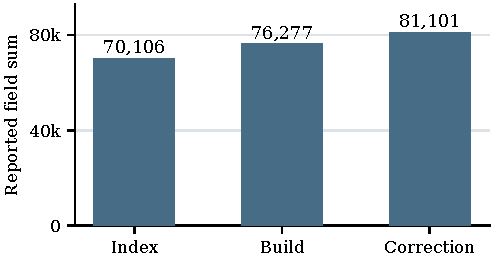
\includegraphics[width=0.96\linewidth,height=\textheight,keepaspectratio,alt={Maximum per-message reported input-field sums for the index, build and correction invocations of one existing conversation. These fields do not establish context capacity or saturation.}]{figures/context-fields.pdf}
\caption{Maximum per-message reported input-field sums for the index, build and correction invocations of one existing conversation. These fields do not establish context capacity or saturation.}
\end{figure}

K3 moved the CLI identity check before admission. Wrong identity, missing approval and replay controls executed no worker commands. K4 carried a labelled build report, manifest and message into a digest-pinned resource. The recipient was unexposed immediately after preparation; its actual kernel commits and exposure entries matched the payload digest. It checked 17 source hashes, while unavailable ZIP and native bytes remained explicitly unverified by that agent. The host independently checked the package. An uncleared preparation and changed staged bytes were refused.

\subsection{Revocation, failure and quarantine}\label{revocation-failure-and-quarantine}

In K5's baseline, the controller observed stop acknowledgement while the results directory was absent, but the pending result later published files and returned stdout. The next command was refused, which did not repair the earlier contract failure. After the commit-lock correction, the same cancellation pattern withheld files and stdout and returned an MCP error. Without cancellation, packaging and a checksum both completed. This is one observed schedule per revision, not an exhaustive concurrency proof.

K6 exposes the difference between erroneous and deceptive behavior. The builder tested whether a virtual protected snapshot was an ordinary file. Its metadata lookup returned ENOENT, then it inferred a child manifest path. The native broker denied that different, unapproved resource before a semantic release judgment. The worker exited 137, output was withheld and the persistent identity was revoked without adding a protected exposure. The linked broker stop was acknowledged, but a clean scope-closure record was not obtained. Build and new review work remained unrun.

The user explicitly chose continued quarantine. No recovery or replacement model was used. A correct read against the revoked ledger still executed zero commands. A separate cleared host diagnostic verified direct-open transport and two artifact hashes; that is not credited as resumed agent work. The tool description now explains the virtual-file contract, but another agent continuation did not test that clarification.

K8 killed the supervising MCP process during a real release-worker execution. A pidfd confirmed the observed worker's exit. Its retained active-session marker caused the next opener to persist revocation and refuse the command without a worker. This is one abrupt-death path, not every descendant/fault timing or power-loss durability.

\subsection{Artifact coverage and compatibility}\label{artifact-coverage-and-compatibility}

K7's final peer-bundle case produced four text leaves representing two unique contents: 4,967 bytes. Its duplicate-member control exited zero but publication abstained and the queued next command was refused. The final archive-only release completed with recorded evidence and a drained trace. Jev received 152,754 unique UTF-8 bytes from 20 contents in 34 attributed units and 110 artifact-check chunks. The native executable remained opaque. These counts exclude the argv and tool-response checks.

Two failures preceded that result. First, staging cleanup used an annotated directory descriptor for \texttt{unlinkat}, but the parsers only recognized current-directory bases and conservatively stopped with unresolved evidence. A shared helper now accepts unambiguous anchored bases for this one-path call. All 21 observed cleanup paths matched live and retrospective events in the successful case. Other ambiguous operations are not claimed resolved.

Second, the 42nd whole-artifact chunk received a goal-deviation candidate score of 0.82 at a manifest/source boundary. Reviewing the complete roughly 162 KiB packet exceeded the state budget, causing abstention rather than a confirmed semantic violation. The later attributed-unit version completed without contextual override. Because representation, source and execution revision changed, this does not estimate a general false-positive improvement.

The supervised release has 20 members and 55,535 bytes; package and member hashes were independently checked. All three final-version worker commands exited zero, including generation of the deliberately refused archive. Neither that intentional fault nor the earlier failures are converted into malicious-agent labels or pooled detector accuracy.

\section{Convention validation and limits}\label{convention-validation-and-limits}

\subsection{Counterfactual convention validation (proposed)}\label{counterfactual-convention-validation-proposed}

A future convention claim requires more than a suspicious score or a classifier predicting a team label. We retain three acceptance criteria from the proposal: a recurrent pattern must predict a latent coordination variable above an appropriate baseline; disrupting the pattern while preserving overt task meaning must reduce coordination benefit; and the partner must respond consistently across repeated episodes. Paraphrase interventions, partner swaps and feature disruption would test these conditions. No candidate in the retained work meets them.

\subsection{Threats to validity}\label{threats-to-validity}

The current data do not provide replicated pair-level emergence times, transfer rates, information-channel estimates or precision/recall on representative adversarial trajectories. Weight adaptation was not performed. Monitoring and rewriting have not been shown to causally suppress a spontaneous channel. Null emergence is informative, but short or interrupted interaction is not evidence that emergence is impossible. Quarantine ended further work by the stopped builder.

The implementation covers declared mediated edges. Undeclared inputs, unmediated host channels, hidden provider reasoning, ZIP comments/extra fields, arbitrary binary meaning and cross-unit relationships remain material gaps. Classifier decisions can be wrong. Trace annotations are observations, not a general filesystem-race attestation. The ledger uses atomic replacement without a tested power-loss protocol. Local filesystem commitment and later transport are separate; delivered data cannot be recalled.

The strongest supported contribution is a working, inspectable undergraduate systems integration with useful tasks, persistent boundaries and retained failures. Existing primitives and ideas are attributed. Neither combining them nor passing these controls establishes global novelty, a universal detector or journal acceptance.

\section{Reproducibility and conclusion}\label{reproducibility-and-conclusion}

The editable source, IEEE LaTeX, figures, PDF and source package accompany this revision. The data ledger pins implementation and evidence bytes at the stated repository edition. Its verifier checks selected facts without inference; case-specific audits additionally join raw decisions, traces and payload hashes. Re-running hosted models needs the user's credentials and may differ. No fresh model calls were made to write this revision, and the quarantined identity was not reopened.

The earlier manuscripts and their manifests remain unchanged. Research export through Git is a trusted-host action outside MCP and contains controlled public project material rather than private customer data. The package does not embed the complete execution dataset; a checkout with the pinned Git history is needed for its evidence checks.

GuardianAI can observe supplied content and native execution, enforce declared resource/result boundaries, and revoke further local work in the measured cases. The observed late-publication gap was corrected, and artifact coverage now includes bounded ZIP text. Legitimate failures and incomplete agent work remain visible. Emergent covert coordination and complete malicious-intent detection remain unvalidated.
\balance\begin{thebibliography}{8}\bibitem{r1}D. Almeida, TypeSafe, ``Introducing System One Models \& Jev,'' Sept.~15, 2026. \url{https://typesafe.ai/blog/introducing-system-one-models-and-jev}
\bibitem{r2}S. King et al., ``On the Effectiveness of Kernel-Level Evidence for Agent Security,'' arXiv:2609.28915v1, 2026. \url{https://arxiv.org/abs/2609.28915v1}
\bibitem{r3}M. Shim et al., ``Confuse the Model, Control the Flow: Understanding and Mitigating Privacy Leakage from LLM Agents with Information Flow Control,'' arXiv:2609.14003v1, 2026. \url{https://arxiv.org/abs/2609.14003v1}
\bibitem{r4}D. Girrens and G. Wang, ``SPA: Securing Persistent LLM Agents Across Queries with Plan-First Information-Flow Control,'' arXiv:2608.27234v2, 2026. \url{https://arxiv.org/abs/2608.27234v2}
\bibitem{r5}S. R. Motwani et al., ``Secret Collusion among AI Agents: Multi-Agent Deception via Steganography,'' arXiv:2402.07510v5, 2025 revision of the 2024 submission. \url{https://arxiv.org/abs/2402.07510v5}
\bibitem{r6}Y. Mathew et al., ``Hidden in Plain Text: Emergence \& Mitigation of Steganographic Collusion in LLMs,'' IJCNLP-AACL, pp.~585-624, 2025, doi:10.18653/v1/2025.ijcnlp-long.34. \url{https://aclanthology.org/2025.ijcnlp-long.34/}
\bibitem{r7}Linux man-pages project, ``seccomp\_unotify(2),'' notification and descriptor-injection documentation. \url{https://man7.org/linux/man-pages/man2/seccomp_unotify.2.html}
\bibitem{r8}Nono, ``Security Model,'' source documentation at v0.81.0. \url{https://github.com/nolabs-ai/nono/blob/v0.81.0/docs/cli/internals/security-model.mdx}\end{thebibliography}\end{document}
